
\subsection{Chernoff Bounds}
The method to derive Chernoff bounds is nearly identical to the method used to derive Hoeffding's inequality. The sole difference is that the MGF is bounded by the inequality $1+x \leq e^x$ instead of $\frac{e^x + e^{-x}}{2} \leq e^{x^2/2}.$ \\ 

\begin{tcolorbox}
\begin{theorem}[Chernoff Inequality]
Suppose $X1, .., X_N$ are independent Bernoulli random variables with probabilities $p_1, ..., p_N$ with $S_N = \sum_{i=1}^{N}X_i$ and $E[S_N] = \mu$, then
    \begin{equation}
    P(S_n \geq t) \leq e^{-\mu}\left(\frac{e \mu}{t}\right)^t
    \label{eq:chernoff1}
    \end{equation}
Alternatively, for $\delta \in (0,1],$ the Chernoff Inequality may be written as 
    \begin{equation}
    P\left(|S_n-\mu| \geq \delta \mu \right) \leq 2e^{-c \mu \delta^2}
    \label{eq:chernoff2}
    \end{equation}
\label{theorem:chernoff}
\end{theorem}
\end{tcolorbox}

\begin{proof}
\begin{align*}
    P(S_n \geq t) &= P\left(\sum_{i=1}^{N}X_i \geq t\right) \\
    &= P\left(\lambda\sum_{i=1}^{N}X_i \geq \lambda t\right) &&\text{multiply both sides by $\lambda$} \\
    &= P\left( \exp\left\{\lambda\sum_{i=1}^{N}X_i\right\} \geq 
        \exp\left\{\lambda t \right\} \right) && \text{exponentiate both sides} \\
    &\leq \frac{E\left[\exp\left\{\lambda \sum_{i=1}^{N}X_i \right\}\right]}{\exp\left\{ \lambda t \right\}} &&\text{Apply Markov's inequality} \\ 
    &\leq \frac{\prod_{i=1}^{N} E\left[\exp\left\{\lambda X_i \right\}\right]}{\exp\left\{ \lambda t \right\}} &&\text{} \\ 
\end{align*}

For a single RV $X_i$, we have 
\begin{align*}
E\left[e^{\lambda X_i}\right] &= (1-p_i) e^{(\lambda)(0)} + p_i e^{ (\lambda)(1) } &&\text{Expectation of Bernoulli RV} \\ 
&= 1 - p_i + p_i e^{\lambda} &&\text{} \\
&= 1 + p_i(e^\lambda - 1) \\
&\leq \exp\left\{ p_i(e^\lambda - 1) \right\} &&\text{since $1+x \leq e^x$} \\
\end{align*}

Returning to the full proof, we have 
\begin{align*}
    P(S_n \geq t) &\leq \frac{\prod_{i=1}^{N} E\left[\exp\left\{\lambda X_i \right\}\right]}{\exp\left\{ \lambda t \right\}} &&\text{} \\ 
    &\leq \frac{ \prod_{i=1}^{N} \left[ \exp\{p_i(e^\lambda - 1)\} \right] }{\exp\{\lambda t\}} &&\text{since $E[e^{\lambda X_i}] \leq \exp\{p_i(e^\lambda - 1)\}$}\\
    &= \exp\{-\lambda t\}\exp\left\{ \sum_{i=1}^{N}p_i(e^\lambda - 1) \right\} &&\text{product of powers} \\
    &= \exp\{-\lambda t\}\exp\left\{ \mu (e^\lambda - 1) \right\} &&\text{$\sum_{i=1}^{N}p_i = \sum_{i=1}^{N}E[X_i] = E\left[\sum_{i=1}^{N}X_i\right] = E\left[S_n\right] = \mu$} \\
\end{align*}
Searching for the value of $\lambda$ that minimizes this bound, we find that $\lambda = \ln(t/\mu)$. Plugging this into the bound, we find  
\begin{align*}
    e^{-\lambda t} e^{\mu(e^\lambda - 1)} &= \left(\frac{t}{\mu}\right)^{-t} e^{ \mu \left(t/\mu-1\right) } \\
    &= \left(\frac{\mu}{t}\right)^{t} e^{ t-\mu } \\
    &= e^{-\mu} \left( \frac{e \mu}{t} \right)
\end{align*}
That is, 
$$ P(S_n \geq t) = e^{-\mu} \left( \frac{e \mu}{t} \right). $$
\end{proof}




\begin{figure}[H]
\begin{subfigure}{0.5\textwidth}
    \centering
    \begin{tikzpicture}
    \begin{axis}[
        axis lines = center,
        xlabel = $x$,
        ylabel = {$f(x)$},
    ]
    %Below the red parabola is defined
    \addplot [
        domain=-2:2, 
        samples=100, 
        color=red,
    ]
    {e^x};
    \addlegendentry{$e^x$}
    %Here the blue parabloa is defined
    \addplot [
        domain=-2:2, 
        samples=100, 
        color=blue,
        ]
        {1+x};
    \addlegendentry{$1+x$}
    \end{axis}
    \end{tikzpicture}
\end{subfigure}
\begin{subfigure}{0.5\textwidth}
    \centering
    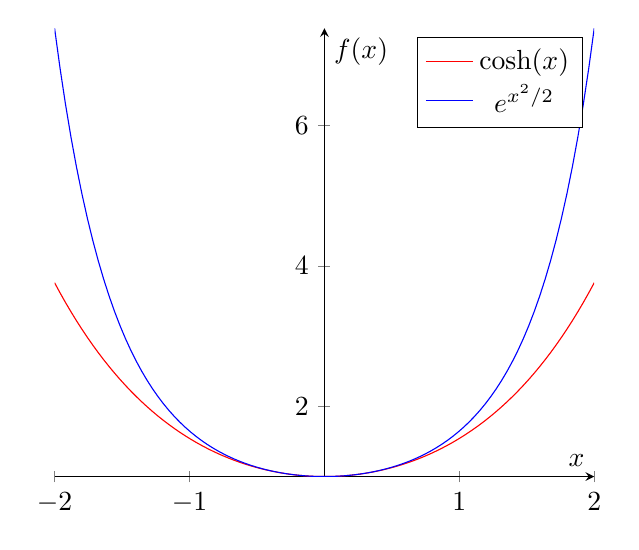
\begin{tikzpicture}
    \begin{axis}[
        axis lines = center,
        xlabel = $x$,
        ylabel = {$f(x)$},
    ]
    %Below the red parabola is defined
    \addplot [
        domain=-2:2, 
        samples=100, 
        color=red,
    ]
    {cosh(x)};
    \addlegendentry{$\cosh(x)$}
    %Here the blue parabloa is defined
    \addplot [
        domain=-2:2, 
        samples=100, 
        color=blue,
        ]
        {exp(x^2/2)};
    \addlegendentry{$e^{x^2/2}$}
    \end{axis}
    \end{tikzpicture}
\end{subfigure}
\end{figure}

% \begin{figure}[H]
%     \centering
%     \begin{tikzpicture}
%     \begin{axis}[
%         axis lines = center,
%         xlabel = $x$,
%         ylabel = {$f(x)$},
%     ]
%     %Below the red parabola is defined
%     \addplot [
%         domain=-2:2, 
%         samples=100, 
%         color=red,
%     ]
%     {x^x};
%     \addlegendentry{$x^x$}
%     %Here the blue parabloa is defined
%     \addplot [
%         domain=-2:2, 
%         samples=100, 
%         color=blue,
%         ]
%         {x};
%     \addlegendentry{$e^{x^2/2}$}
%     \end{axis}
%     \end{tikzpicture}
% \end{figure}



